\documentclass{article}
\usepackage{tikz,times}
\usepackage[paperwidth=25cm,paperheight=22cm,left=1cm,top=1cm]{geometry}

\usetikzlibrary{mindmap,backgrounds,trees}

\pagestyle{empty}

\begin{document}

\centering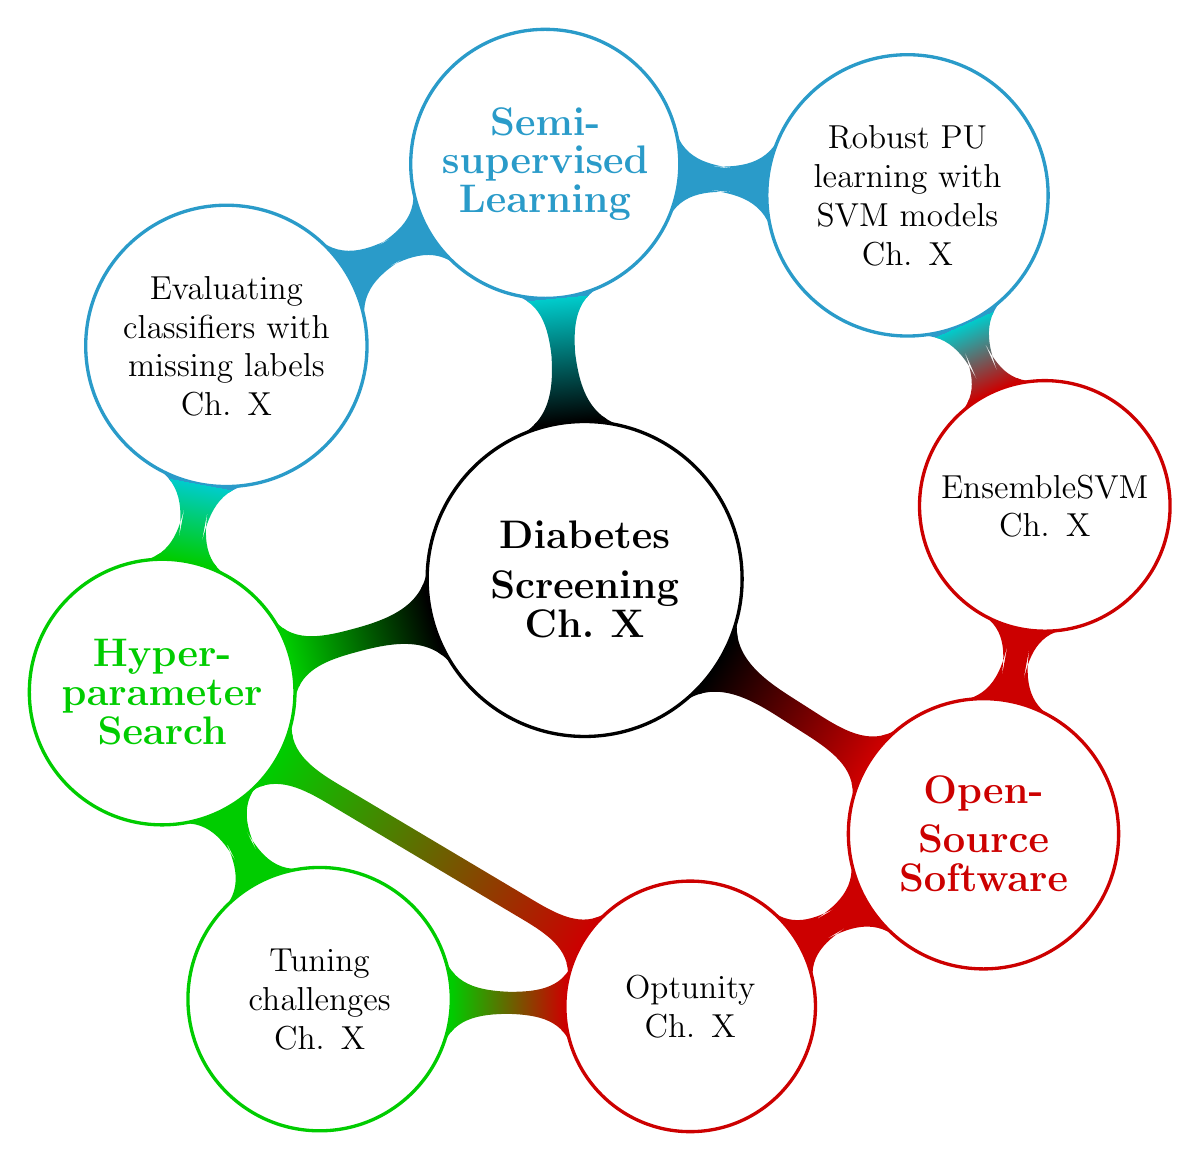
\begin{tikzpicture}[mindmap,
  every node/.style={font=\large},
  every concept/.style={minimum size=3cm, text width=3cm, fill=none, very thick},
  level 1 concept/.append style={level distance=150,sibling angle=120}]

  \begin{scope}[mindmap, text=black, minimum size=3cm]
    \node [concept, minimum size=4cm, color=black, text=black] at (0, 0) {\Large{\textbf{Diabetes Screening \\ Ch. X}}}
	[clockwise from=90, level distance=130] 
	child[concept color=cyan!80!black] {node [concept, text=cyan!80!black] at (-0.5, 0) (pulearning) {\Large{\textbf{Semi-supervised Learning}}}
		[clockwise from=0, sibling angle=180]
		child {node [concept] at (1.7, -0.4) (resvm) {Robust PU learning with SVM models \\ Ch. X}}
		child {node [concept] at (-5.5, 0.2) (evaluation) {Evaluating classifiers with missing labels \\ Ch. X}}
	      }
	child[concept color=red!80!black] {node [concept, text=red!80!black] at (0.5, -0.6) (software) {\Large{\textbf{Open-Source \\ Software}}}
		[clockwise from=200, level distance=200, sibling angle=90]
		child {node [concept] at (-1, -1.2) (optunity) {Optunity \\ Ch. X}}
		child {node [concept] at (3.0, 2.3) (esvm) {EnsembleSVM \\ Ch. X}}
	      }
	child[concept color=green!80!black]{node [concept, text=green!80!black] at (-0.8, 1.2) (tuning) {\Large{\textbf{Hyper-parameter Search}}}
		[clockwise from=270, level distance=200, sibling angle=90]
		child {node [concept] at (2, -1) (mic) {Tuning challenges \\ Ch. X}}
	      };
  \end{scope}

\path (resvm) to[circle connection bar switch color=from (cyan!80!black) to (red!80!black)] (esvm) ;
\path (tuning) to[circle connection bar switch color=from (green!80!black) to (red!80!black)] (optunity) ;
\path (mic) to[circle connection bar switch color=from (green!80!black) to (red!80!black)] (optunity) ;
\path (tuning) to[circle connection bar switch color=from (green!80!black) to (cyan!80!black)] (evaluation) ;

\end{tikzpicture}


\end{document}
